\section{Visão computacional}

A visão computacional está em constante avanço, aproximando cada vez mais os computadores da capacidade visual humana. De acordo com Horst Haußecker e Bernd Jähne, no livro "Computer Vision and Applications" \cite{comp_vision_and_applications}, a visão computacional é uma área da computação que se dedica à interpretação de imagens por meio de algoritmos e técnicas de processamento de imagens. Essa área abrange a aquisição, processamento e análise de imagens, com o objetivo de extrair informações úteis para resolver problemas específicos.

Porém, segundo Richard Szeliski, no livro "Computer Vision: Algorithms and Applications" \cite{computer_vision_richard}, nas últimas décadas ocorreram avanços significativos na busca de aproximar a visão computacional da visão humana, porém não obteve total êxito. Isso ocorre porque, enquanto o olho humano enxerga com aparente facilidade as estruturas tridimensionais e suas nuances, a visão computacional depende de técnicas matemáticas altamente precisas para recuperar a forma tridimensional e a aparência dos objetos.

Nas figuras \cref{fig:imagem_a} e \cref{fig:imagem_b}, evidencia-se a notável capacidade de um computador em distinguir, classificar e até mesmo compreender os elementos presentes em uma fotografia.

\begin{figure}
    \centering
    \begin{minipage}[b]{0.49\textwidth}
      \centering
      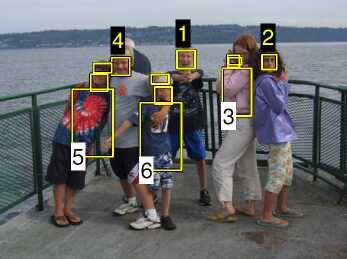
\includegraphics[width=0.6\textwidth]{figures/detectacao_de_faces_exemplo.JPG}
      \caption{Algoritmos de detecção facial e de roupas/cabelos por cor localizam e reconhecem pessoas nesta imagem \cite{computer_vision_richard}}
      \label{fig:imagem_a}
    \end{minipage}
    \hfill
    \begin{minipage}[b]{0.49\textwidth}
      \centering
      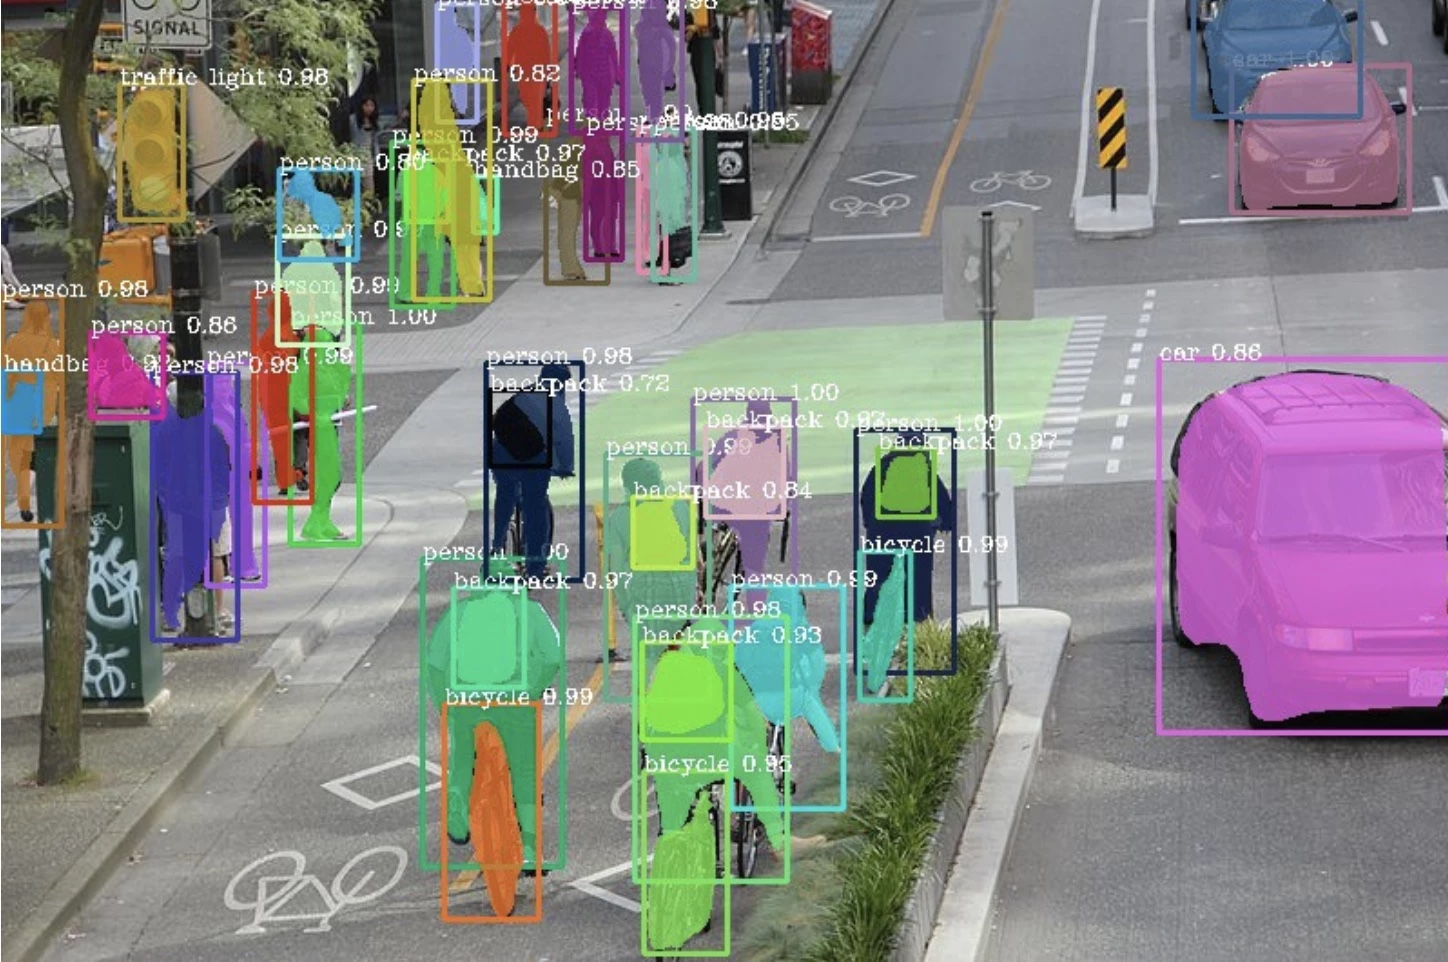
\includegraphics[width=0.6\textwidth]{figures/semantic_intance.JPG}
        \caption{Segmentação de instâncias de objetos pode delinear cada pessoa e objeto em uma cena complexa. 
        \cite{instance_segmentation}}
      \label{fig:imagem_b}
    \end{minipage}
  \end{figure}


No entanto, apesar do sucesso no uso dessas técnicas, o computador ainda não consegue oferecer a mesma quantidade de detalhes na explicação de uma imagem como o olho humano. Isso se deve à maior facilidade do computador em compreender linguagem em comparação à visualização. A tarefa de ensinar um computador a ver e descrever com precisão e riqueza de detalhes o que está sendo observado é extremamente complexa \cite{computer_vision_richard}.

A visão é um elemento crucial para capacitar a inteligência artificial a realizar diversas tarefas. A fim de replicar a visão humana, é necessário que as máquinas sejam capazes de adquirir, processar, analisar e compreender imagens. \cite{como_funciona_visao_computacional}

% Na \cref{fig:comp_vision} podemos ver uma analogia entre a forma como uma imagem é processada pelo cérebro humano e a forma como é processada por um sistema computacional.

% \begin{figure}[!ht]
% 	\centering
% 	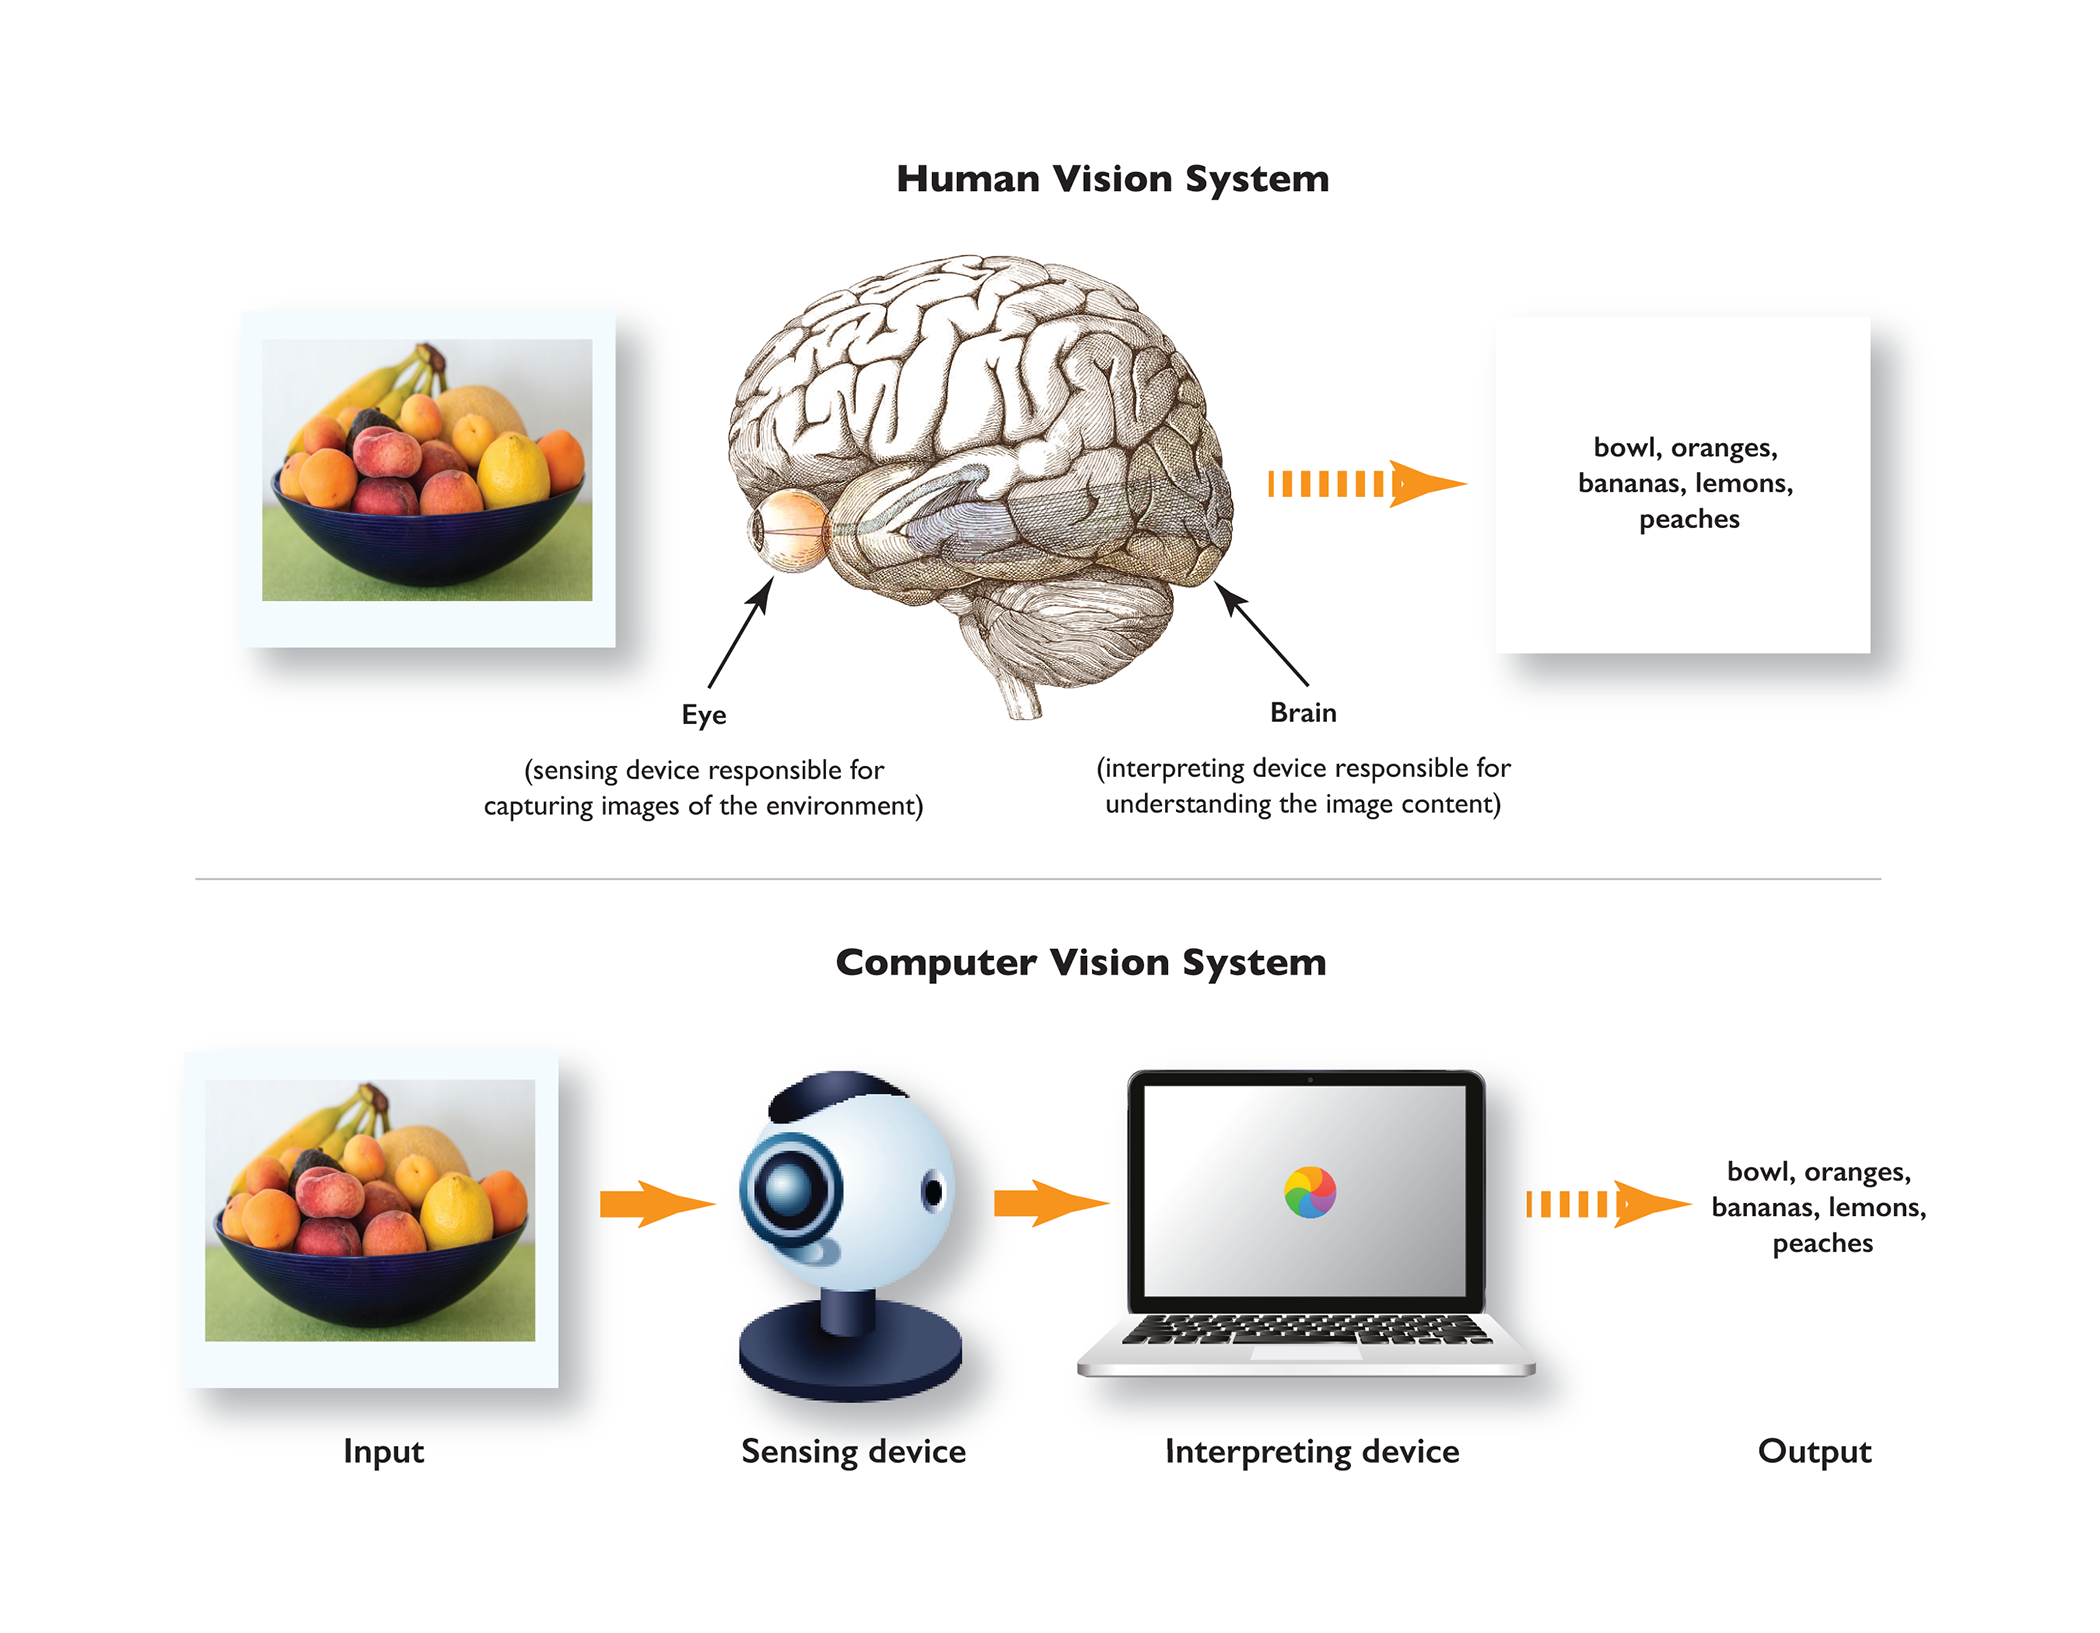
\includegraphics[width=0.6\textwidth]{figures/content_Human_Vision.png}
% 	\caption{Visão humana e sistemas de visão computacional processam dados visuais de maneira semelhante \cite{content_Human_Vision}.}
% 	\label{fig:comp_vision}
% \end{figure}	


\subsection*{Como a visão computacional funciona?}

No processamento de computação visual, as imagens são adquiridas e representadas como uma matriz 2D de pixels. Cada pixel corresponde a um ponto na imagem e é representado por um valor numérico que varia de 0 a 255. Esses valores de pixel descrevem a intensidade da cor em uma escala de cinza. Dessa forma, um computador interpreta uma imagem como uma matriz de números, permitindo que ele analise e compreenda os detalhes visuais presentes na imagem, como no caso da \cref{fig:comp_vision} do presidente dos Estados Unidos, Abraham Lincoln\cite{mit_video}.

Os algoritmos de visão computacional utilizados atualmente são fundamentados em reconhecimento de padrões. O procedimento consiste em treinar computadores por meio de uma vasta quantidade de dados visuais. Os computadores processam imagens, rotulam os objetos nelas contidos e identificam padrões entre esses objetos \cite{content_Human_Vision}.

Esse processo de treinamento e reconhecimento de padrões permite que os computadores identifiquem objetos e compreendam seu contexto visual. Com essa capacidade, o computador consegue realizar tarefas como, por exemplo, reconhecimento facial \cref{fig:imagem_a}.

\begin{figure}[!ht]
	\centering
	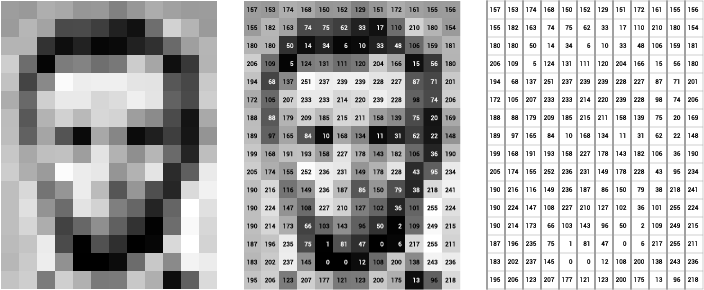
\includegraphics[width=0.6\textwidth]{figures/lincoln_pixel_values.png}
	\caption{Diagrama de dados de pixels. À esquerda, nossa imagem de Lincoln; no centro, os pixels rotulados com números de 0 a 255, representando sua luminosidade; e à direita, apenas esses números \cite{content_Human_Vision}.}
	\label{fig:comp_vision}
\end{figure}



